\documentclass[UTF8,zihao=-4]{ctexart}

% =======================
% 基本页面设置
% =======================
\usepackage[a4paper,margin=2.5cm]{geometry}
\usepackage{setspace}
\onehalfspacing

% =======================
% 数学与表格
% =======================
\usepackage{amsmath,amssymb,amsfonts,bm}
\usepackage{booktabs}
\usepackage{threeparttable}
\usepackage{tabularx}
\usepackage{longtable}
\usepackage{array}
\usepackage{multirow}
\usepackage{makecell}

% =======================
% 图形与浮动体
% =======================
\usepackage{graphicx}
\usepackage{float}
\usepackage{subcaption}
\usepackage{caption}
\captionsetup{font=small,labelfont=bf}

% =======================
% 引用与超链接
% =======================
\usepackage[authoryear,round]{natbib}
\usepackage[colorlinks=true,
            linkcolor=black,
            citecolor=blue,
            urlcolor=blue]{hyperref}

% =======================
% 其他
% =======================
\usepackage{enumitem}
\usepackage{xcolor}
\usepackage{siunitx}
\usepackage{indentfirst}
\setlength{\parindent}{2em}

% =======================
% 论文信息
% =======================
\title{}
\author{}
\date{}

\begin{document}

% =======================
% 首页标题信息：不单独占页
% =======================
\begin{center}
    {\zihao{2}\heiti 货币政策冲击与行业资产定价：}\\[0.4em]
    {\zihao{3}\heiti 基于FOMC事件窗口和Fama-French行业组合的经验证据}\\[1.2em]
    {\zihao{-4} 刘师妤}\\[0.3em]
    {\zihao{-4} 学号：2024201568}
\end{center}

\vspace{0.8em}


% =======================
% 摘要
% =======================
\begin{abstract}
本文围绕FOMC货币政策冲击对美国行业资产价格的异质性影响展开研究。
% 研究问题 -> 数据方法 -> 主要发现 -> 谨慎口径
% 这里不需要详细写住房市场SEM，只在一句话中说明本文还从联立方程角度补充讨论货币政策传导中的识别问题。
\end{abstract}

\noindent\textbf{关键词：} FOMC；货币政策冲击；行业资产定价；利率脆弱度；事件研究；异质性反应

% =======================
% 1 Introduction
% =======================
\section{引言}

% 1. 现实背景：FOMC 是重要宏观信息事件。
% 2. 简短 related work：货币政策冲击、资产定价、行业异质性。
% 3. 研究缺口：已有讨论更多关注整体市场，本文关注行业截面。
% 4. 研究问题：鹰派 FOMC 是否使高利率脆弱行业表现更差。
% 5. 数据与方法预告：49 行业、FOMC、DGS2、OLS、IV、面板、限值模型。
% 6. 主要发现与贡献。

FOMC 公告往往是金融市场重新定价的重要时点。一次政策声明或新闻发布会并不只是告诉市场当前联邦基金目标利率是否变化，更重要的是改变投资者对未来利率路径、通胀压力、经济增长和风险偏好的判断。短端利率会首先反映这些预期修正，而股票价格则会通过折现率、风险溢价、融资成本和未来现金流预期等渠道迅速调整。已有货币政策资产定价研究表明，金融市场会对货币政策意外作出显著反应，尤其是股票市场收益与政策利率意外之间存在系统性联系 \citep{kuttner2001monetary,bernanke2005stock}；同时，FOMC 声明和沟通本身也包含重要信息，政策行动和政策沟通都可能改变资产价格 \citep{gurkaynak2005actions}。

不过，市场指数的平均反应只揭示了货币政策冲击的一部分。现实中，同一次 FOMC 公告之后，不同行业的收益表现经常出现明显分化。利率上升预期可能压低长久期现金流的现值，也可能提高外部融资依赖行业的债务成本，还可能通过耐用品消费、住房需求和企业投资影响周期性行业。房地产、汽车、建筑材料、公用事业、耐用品和金融相关行业通常具有较强的利率敏感性；黄金等行业还可能同时受到通胀预期、避险需求和美元走势影响。因此，货币政策冲击并不是均匀作用于全部股票，而是可能沿着行业融资结构、现金流久期、需求弹性和风险暴露形成截面差异。

这正是本文关注的问题：在 FOMC 公告事件窗口内，历史上对利率变化更敏感的行业，是否会在更强紧缩性政策信号出现后产生更低的事件窗口收益或异常收益，并进一步面临更高的下行风险？这个问题不同于传统的市场层面事件研究。市场层面研究回答的是“货币政策是否影响整体股票市场”；本文进一步追问的是，在同一个宏观信息冲击下，为什么有些行业受到更强冲击，而另一些行业反应较弱。换言之，本文把货币政策事件研究和行业截面资产定价结合起来，考察政策利率预期修正如何通过行业利率脆弱度转化为资产价格的相对变化。

这一问题也带来一个基本的计量要求：不能只比较高低利率脆弱行业的平均收益。行业事件窗口收益本身会受到市场风险、规模、价值、盈利能力、投资风格、历史波动和事件前动量等因素影响。资产定价文献已经表明，股票收益具有系统性风险因子结构，市场、规模、价值、盈利能力和投资因子均可能解释横截面收益差异 \citep{fama1993common,fama2015five}。因此，如果利率脆弱行业同时也是高波动、高成长或具有特殊避险属性的行业，简单相关关系就可能混入遗漏变量偏误。本文的实证设计由此从最简单的事件窗口截面回归出发，逐步加入资产定价因子暴露和行业收益特征控制变量，并进一步讨论异方差、影响点、测量误差和工具变量等识别问题。

具体而言，本文的研究设计分为三个层次。第一，本文以 2022 年快速加息周期中的典型 FOMC 事件为起点，构造 49 个行业组合的事件窗口收益和历史利率脆弱度，先用简单截面 OLS 刻画二者之间的基本关系。第二，本文在截面模型中加入 Fama-French 因子暴露、历史波动率和事件前动量等控制变量，估计控制行业风险特征后的利率脆弱度偏效应，并通过异方差稳健标准误、WLS/FGLS、影响点诊断、代理变量和工具变量辅助检验讨论结果的稳健性与识别边界。第三，本文将样本扩展到 2017--2026 年多次 FOMC 会议构成的行业--事件面板，使用连续暴露双向固定效应、2022 年政策环境变化、公告窗口 DID/DDD 以及限值因变量模型，进一步检验货币政策冲击是否表现为行业间相对重定价和下行风险上升。

相对于主要关注市场指数平均反应的货币政策事件研究，本文的边际贡献在于把 FOMC 冲击放到行业截面结构中考察。这个视角使我们能够观察同一政策信息如何沿着行业利率暴露产生相对重定价，而不是只看到市场整体涨跌。同时，本文将事件研究和资产定价控制变量结合起来，区分单纯相关关系与控制行业风险特征后的偏效应；并进一步把结果变量从平均事件窗口收益扩展到跑输概率、负异常收益天数和下行损失，从而补充刻画紧缩性政策信号下的行业下行风险。后文将依次展开理论机制与研究假设、数据和变量构造、基准回归、稳健性与内生性讨论、异质性和机制检验，给出政策建议，并在最后总结研究结论与不足。

\section{理论基础、文献综述与研究假设}

\subsection{货币政策冲击与股票市场反应}

股票价格本质上反映了投资者对未来现金流及其折现率的综合定价。FOMC公告是金融市场重新修正宏观预期的重要时点：一方面，政策声明、点阵图和新闻发布会会改变市场对未来短端利率路径的判断；另一方面，货币政策沟通也会同时传递关于通胀压力、经济增长和金融风险偏好的信息。因此，FOMC公告并不只是“是否加息”的离散事件，而是包含了市场对未来货币条件重新定价的连续信息冲击。

已有研究通常采用事件研究法识别货币政策冲击对金融资产价格的即时影响。该方法的核心思想是：如果公告窗口足够短，窗口内资产收益的异常变化更可能来源于公告信息本身，而不是其他缓慢变化的基本面因素。Kuttner \citep{kuttner2001monetary} 利用联邦基金期货刻画未预期的货币政策变动，发现 Interest Rate Surprise (利率意外)是理解资产价格反应的关键；Bernanke and Kuttner \citep{bernanke2005stock} 进一步表明，股票市场会对货币政策意外产生显著反应；Gürkaynak et al. \citep{gurkaynak2005actions} 则强调，FOMC沟通不仅包含当前政策行动，还包含未来政策路径的信息。

基于上述思路，本文将FOMC公告视为外生宏观信息集中释放的事件节点，并以公告日前后短窗口内的行业组合事件窗口收益作为核心结果变量：在单事件截面分析中，主要考察行业组合的累计收益或市场调整收益；在多事件面板和扩展检验中，进一步使用因子调整后的累计异常收益。具体而言，设行业 $i$ 在事件窗口 $\mathcal{W}$ 内第 $\tau$ 日的异常收益为
\[
AR_{i\tau}=R_{i\tau}-\widehat{R}_{i\tau},
\]
其中 $R_{i\tau}$ 为行业实际收益，$\widehat{R}_{i\tau}$ 为根据市场模型或资产定价因子模型预测的正常收益。行业 $i$ 的累计异常收益定义为
\[
CAR_i=\sum_{\tau\in \mathcal{W}} AR_{i\tau}.
\]
在后续实证中，本文关注的问题并不是“FOMC公告是否影响全部股票市场”，而是进一步考察：在同一次鹰派政策冲击后，不同行业是否由于利率脆弱度不同而表现出系统性的横截面差异。

\subsection{行业利率脆弱度与货币政策传导机制}

货币政策对股票市场的影响具有明显的行业异质性。即使同一次FOMC公告对所有行业同时发生，不同行业的现金流结构、融资方式、需求弹性和资产久期不同，也会导致其收益反应存在差异。本文所说的“行业利率脆弱度”，是指行业收益对利率上升或鹰派货币政策冲击的敏感程度。在实证构造中，行业利率脆弱度主要由历史窗口内行业收益对2年期美债收益率变化的负向敏感度估计得到，数值越高表示利率上升时行业收益越容易受到压制。利率脆弱度越高的行业，在紧缩性政策信息出现后，理论上越容易出现更低的异常收益。

第一，贴现率渠道会直接影响高久期行业的估值。根据资产定价的基本逻辑，股票价格可以理解为未来现金流的折现值。当市场预期未来无风险利率上升时，折现率提高，远期现金流占比较高的行业估值受到更强冲击。成长性更强、盈利兑现更靠后的行业，往往具有更高的现金流久期，因此对利率变化更加敏感 \citep{cochrane2005asset}。

第二，融资成本渠道会影响依赖外部融资的行业。鹰派FOMC公告通常意味着未来金融条件可能趋紧，企业债务融资成本和权益融资成本上升。对于杠杆率较高、投资支出较大或现金流较不稳定的行业，融资成本上升会压缩投资和经营空间，从而降低市场对其未来盈利的预期。该机制与货币政策传导中的信贷渠道和资产负债表渠道一致 \citep{mishkin1996channels,bernanke1995inside}。

第三，需求收缩渠道会影响利率敏感型消费和投资需求。货币政策紧缩不仅作用于企业融资端，也会影响居民消费、房地产、耐用品购买和企业资本开支。因而汽车、建筑、房地产相关产业链、资本品等行业可能通过终端需求下降而受到更大影响。

第四，风险偏好渠道会放大行业间差异。鹰派政策信息通常会降低市场风险偏好，提高投资者要求的风险补偿。在这种环境下，市场可能从高波动、高估值或高融资依赖行业撤出，转向现金流更稳定、防御属性更强的行业。由此，利率脆弱度不仅反映单一的利率暴露，也综合体现了贴现率、融资约束、需求敏感性和风险溢价变化共同作用下的行业脆弱性。

\subsection{资产定价控制变量与事件窗口收益度量}

为了将行业利率脆弱度的影响与其他常见资产定价特征区分开，本文在基准回归之外进一步加入行业风险暴露和历史收益特征作为控制变量。计量上，这一步对应多元线性回归中的“其他条件不变”思想：在控制市场风险、规模、价值、盈利、投资、历史波动和事件前动量后，核心解释变量的系数刻画的是行业利率脆弱度对异常收益的条件相关或偏效应，而不是简单相关关系。

首先，本文控制市场风险暴露。市场$\beta$较高的行业本身就更容易在宏观事件中产生更大波动，如果不控制市场风险，利率脆弱度系数可能混入一般系统性风险的影响。其次，本文控制Fama-French因子暴露，包括规模因子、价值因子、盈利因子和投资因子等。Fama and French \citep{fama1993common,fama2015five} 表明，不同股票组合收益可以由若干系统性风险因子解释；若行业利率脆弱度与这些因子暴露相关，遗漏这些变量会导致核心系数解释不清。再次，本文控制历史波动率和事件前动量。历史波动率反映行业自身风险水平，事件前动量则用于缓解公告前市场已经部分定价或行业短期趋势差异带来的干扰。

因此，本文的核心截面回归可概括为：
\[
CAR_i=\alpha+\beta RateVulnerability_i+\boldsymbol{\gamma}'\mathbf{X}_i+\varepsilon_i,
\]
其中 $CAR_i$ 为行业 $i$ 在FOMC事件窗口内的累计异常收益，$RateVulnerability_i$ 为行业利率脆弱度，$\mathbf{X}_i$ 表示市场风险暴露、Fama-French因子暴露、历史波动率和事件前动量等控制变量。若 $\beta<0$，则说明在控制其他行业特征后，利率脆弱度更高的行业在鹰派FOMC公告后表现更弱。

需要强调的是，本文并不将单一横截面OLS系数机械解释为完全结构性的因果效应。FOMC公告的事件窗口设计有助于减少反向因果和长期遗漏变量的影响，但行业特征仍可能与不可观测因素相关。因此，后文将通过增加控制变量、采用异方差稳健标准误、进行异方差统计检验、影响点诊断、替换事件窗口和被解释变量、代理变量检验以及工具变量/2SLS辅助分析，检验结果的稳健性和识别边界。

\subsection{研究假设}

基于上述理论机制，本文提出以下研究假设。

\textbf{H1 直接影响假设：} 在鹰派FOMC公告后，利率脆弱度更高的行业具有更低的累计异常收益或平均异常收益。换言之，若行业收益对利率上升更敏感，则在政策路径被重新定价为更紧缩时，该行业应出现更明显的负向价格调整。

\textbf{H2 偏效应假设：} 在控制市场风险暴露、Fama-French因子暴露、历史波动率和事件前动量后，行业利率脆弱度仍然对事件窗口异常收益具有负向偏效应。该假设关注的不是原始相关关系，而是在其他可观测行业特征保持不变时，利率脆弱度是否仍具有独立解释力。


\textbf{H3 机制渠道假设：} 行业利率脆弱度反映了贴现率暴露、融资约束、需求利率敏感性和风险偏好变化等多重渠道。若该机制成立，则高成长、高波动或融资依赖更强的行业，在鹰派FOMC公告后应表现出更强的负向收益反应。受事件窗口长度和行业层面中介变量可得性的限制，本文不将上述渠道设定为严格的中介效应模型，而是通过机制代理变量及其与利率脆弱度的交互项，考察这些理论渠道是否与经验结果方向一致。


\textbf{H4 冲击放大假设：} 在多次FOMC公告构成的行业--事件面板中，当公告窗口内市场利率冲击更鹰派时，高利率脆弱行业相对于低利率脆弱行业应表现出更弱的异常收益。该假设强调，货币政策资产定价效应不仅取决于FOMC是否实际加息、降息或暂停，也取决于公告引发的市场预期修正。本文将通过行业固定效应、事件固定效应以及政策冲击与行业利率脆弱度的交互项，检验这一跨事件的冲击放大效应。

\textbf{H5 风险状态假设：} 鹰派FOMC公告后，高利率脆弱行业不仅平均收益更低，也更容易进入不利风险状态。具体表现为：更高概率跑输市场或行业基准、更多负异常收益天数，以及更大的下行损失。该假设将被用于连接连续型收益回归与二值、计数和下行风险变量的扩展检验。

% =======================
% 3 数据来源、变量构造与现状分析
% =======================
\section{数据来源、变量构造与现状分析}

本文以表格形式列出因变量、自变量、调节变量、机制代理变量和控制变量，并说明主要数据来源。需要说明的是，代码中还生成了若干交互项、稳健性变量、工具变量和诊断变量，这些变量将在后文相应模型中解释；本节变量表只列论文主实证需要理解的核心变量。

\subsection{数据来源与样本范围}

本文的主实证数据包括四类。第一，\textbf{行业收益}来自 Kenneth French Data Library 的 49 Industry Portfolios 日度收益 \cite{kenFrench49Daily}。第二，\textbf{资产定价控制变量}来自 Fama--French 五因子日度数据 \cite{kenFrenchFF5Daily}。第三，\textbf{利率变量}使用 2 年期美国国债收益率 DGS2，来源为 Federal Reserve H.15 或 FRED \cite{federalReserveH15,fredDGS2}。第四，\textbf{FOMC 事件日期和政策声明}来自 Federal Reserve FOMC calendar and statements \cite{federalReserveFOMCCalendar}；其中 2022 年 11 月 2 日 FOMC 会议作为单事件截面分析的核心事件 \cite{federalReserveFOMC20221102}。

样本分为三个层次。单事件截面分析使用 2022 年 11 月 2 日 FOMC 公告前后 $[-1,+1]$ 交易日窗口，样本为 49 个行业组合。多事件面板分析使用 2017 年 2 月 1 日至 2026 年 4 月 29 日的 74 次常规 FOMC 会议，形成 49 个行业乘以 74 次事件的平衡行业--事件面板，共 3626 个观测。限值因变量模型使用完整 $[-5,+5]$ 公告窗口可得的 73 次事件，行业--事件样本量为 3577。

此外，论文的联立方程方法扩展使用 FRED 月度住房市场数据 \cite{fredHousingSeries}，样本期为 2000 年 1 月至 2024 年 12 月。该扩展仅用于展示供需联立方程和 2SLS 方法，不作为 FOMC 行业收益主线的核心证据。

\subsection{变量构造}

本文核心因变量是 \textbf{FOMC 事件窗口内的行业收益}。单事件截面回归中，$CAR_i$ 表示行业组合在公告窗口内的累计收益：
\[
CAR_i=\sum_{\tau\in\mathcal{W}}R_{i\tau}.
\]
在多事件面板和扩展检验中，本文进一步使用 Fama--French 五因子调整后的 \textbf{异常收益}。设 $\widehat{R}_{i\tau}$ 为根据行业因子暴露预测的正常收益，则异常收益为
\[
AR_{i\tau}=R_{i\tau}-\widehat{R}_{i\tau}.
\]
相应地，累计异常收益为 $AbnormalCAR_i=\sum_{\tau\in\mathcal{W}}AR_{i\tau}$。因此，正文中“\textbf{事件窗口收益}”是总称；当后文讨论多事件面板或公告日前后的日度反应时，若明确说明采用因子调整口径，则该收益变量指的是上述异常收益或累计异常收益。

\textbf{核心自变量}是\textbf{行业利率脆弱度}。具体做法是在历史窗口内对每个行业估计行业超额收益对 Fama--French 五因子和 2 年期美债收益率变化的暴露：
\[
r_{it}-RF_t=\alpha_i+\beta_{M,i}MktRF_t+\beta_{S,i}SMB_t+\beta_{H,i}HML_t
+\beta_{R,i}RMW_t+\beta_{C,i}CMA_t+\beta_{r,i}\Delta DGS2_t+u_{it}.
\]
本文定义 $RateVulnerability_i=-\beta_{r,i}$。如果行业收益在利率上升时下降更多，则 $\beta_{r,i}$ 更负，利率脆弱度更高。回归中使用的是该变量在行业截面上的标准化值 $RateVulnerability_{i}^{z}$。

\textbf{调节变量}用于刻画 FOMC 公告引发的市场利率预期修正。本文使用公告前后三个交易日 2 年期美债收益率变化 $\Delta DGS2_e$ 衡量政策冲击，并将该变化为正的事件定义为\textbf{鹰派冲击} $Hawkish_e$。这不同于\textbf{实际政策动作}：一次实际加息可能已经被市场预期消化，而一次暂停加息也可能因为声明、点阵图或新闻发布会偏紧缩而推高短端利率。

\begin{table}[H]
\centering
\caption{主要变量定义与数据来源}
\begin{threeparttable}
\begin{tabularx}{\textwidth}{p{0.16\textwidth}p{0.20\textwidth}X p{0.22\textwidth}}
\toprule
变量类别 & 变量名称 & 定义与构造 & 数据来源 \\
\midrule
因变量 & 事件窗口收益（$CAR_i$） & 行业在 FOMC 公告窗口内的累计收益，用于衡量公告后的行业价格反应。 & 49 Industry Portfolios \\
因变量 & 异常收益或累计异常收益（$AR_{i\tau}$, $AbnormalCAR_i$） & 用 Fama--French 五因子预测正常收益后得到的调整收益，主要用于多事件面板和公告日前后扩展检验。 & 49 Industry Portfolios；FF5 \\
风险状态因变量 & 跑输、负收益天数和下行损失（$Underperform_{ie}$, $DownDays_{ie}$, $DownsideLoss_{ie}$） & 由事件窗口收益进一步转换得到，用于限值因变量模型，刻画行业是否进入不利风险状态。 & 作者基于行业收益计算 \\
核心自变量 & 行业利率脆弱度（$RateVulnerability_i$） & 行业历史收益对 2 年期美债收益率变化的负向敏感度，标准化后进入回归。 & 49 Industry Portfolios；FF5；DGS2 \\
调节变量 & 鹰派政策冲击（$Hawkish_e$） & FOMC 公告窗口内 2 年期美债收益率上升则取 1，表示市场对未来政策路径作出偏紧缩修正。 & H.15 / FRED DGS2 \\
说明性政策变量 & 实际政策动作（$Action_e$） & 根据目标利率区间变化区分实际加息、降息或暂停，用于和市场利率冲击口径作比较。 & FOMC statements \\
机制代理变量 & 成长性、波动率和行业组指标（$Mechanism_i$） & 用高成长、高波动、黄金、金融、防御性和科技成长行业组等变量代理贴现率、风险偏好和行业异质性渠道。 & 作者基于行业特征构造 \\
控制变量 & 因子暴露（$\mathbf{FactorBeta}_i$） & 行业对市场、规模、价值、盈利和投资因子的历史暴露，用于控制常见资产定价风险特征。 & Fama--French 五因子 \\
控制变量 & 历史波动与事件前动量（$HistVol_i$, $PreMomentum_i$） & 行业历史收益波动率和事件前累计收益，用于控制行业自身风险水平和公告前价格趋势。 & 49 Industry Portfolios \\
\bottomrule
\end{tabularx}
\begin{tablenotes}
\small
\item 注：本文不设定严格的中介效应模型。表中的“机制代理变量”用于检验理论渠道是否与经验结果方向一致，而不是用于识别完整中介效应。
\end{tablenotes}
\end{threeparttable}
\end{table}

\subsection{描述性统计与现状分析}

单事件截面样本包含 49 个行业。2022 年 11 月 2 日 FOMC 事件窗口内，行业累计收益的均值为 $-2.731$，标准差为 $2.948$，最小值为 $-10.620$，最大值为 $4.750$，说明同一次政策公告下行业收益存在明显分化。原始利率脆弱度的均值为 $1.567$，标准差为 $1.581$；标准化后的利率脆弱度均值约为 0，标准差为 1。

多事件样本共包含 74 次常规 FOMC 会议，其中实际加息 18 次、降息 9 次、暂停 47 次。按照 2 年期美债收益率事件窗口变化划分，偏鹰派事件共有 30 次，非鹰派事件共有 44 次。实际政策动作与市场利率冲击并不完全一致：18 次实际加息中只有 7 次被划为偏鹰派冲击，而 47 次暂停会议中有 19 次仍被市场定价为偏鹰派冲击。因此，后文同时报告实际政策动作和市场利率冲击口径，避免把“是否加息”和“是否产生新的紧缩性预期修正”混为一谈。

% =======================
% 4 直接影响分析：基准回归与多元OLS
% =======================
\section{直接影响分析：基准回归与多元 OLS}
\label{sec:direct_effect}

本节考察 2022 年 11 月 2 日 FOMC 公告窗口内，行业历史利率脆弱度是否能够解释行业收益的截面差异。实证分析先给出无控制变量的一元 OLS，用于刻画样本中的原始相关；随后在同一截面上加入市场 beta、Fama--French 风格因子暴露、历史波动率和事件前动量，估计控制可观测行业特征后的偏效应。这样处理的核心不是追求更复杂的模型形式，而是区分两个经验问题：利率脆弱度与公告窗口收益是否存在直接的截面相关，以及该关系在控制常见资产定价风险暴露后是否仍然成立。

\subsection{方法依据：从简单相关到多元偏效应}
\label{subsec:direct_method}

在简单截面模型中，总体关系可写为
\[
Y_i=\beta_0+\beta_1 X_i+u_i,
\]
其中 $\beta_1$ 的解释依赖于误差项 $u_i$ 的性质。按照课程第二讲对简单线性回归的说明，若误差项中包含与 $X_i$ 相关的遗漏因素，则一元 OLS 系数会同时反映核心解释变量和遗漏因素的作用。对应到本文，一元模型中的 $Y_i$ 是行业 $i$ 在 FOMC 事件窗口内的累计收益 $CAR_i$，$X_i$ 是行业的历史利率脆弱度；误差项则可能包含市场 beta、行业风格、历史波动率、事件前收益趋势、行业特殊消息和避险属性等因素。因此，一元 OLS 主要用于建立基准事实，而不能单独承担最终识别结论。

当零条件均值假定可能因为遗漏变量而不满足时，课程第三讲给出的处理方式是将可测度的重要遗漏因素纳入多元线性回归。多元模型的一般形式为
\[
Y_i=\beta_0+\beta_1 X_{1i}+\beta_2 X_{2i}+\cdots+\beta_k X_{ki}+u_i,
\]
其零条件均值假定扩展为
\[
E(u_i\mid X_{1i},X_{2i},\ldots,X_{ki})=0.
\]
在该框架下，$\beta_1$ 的含义不再是简单相关，而是在其他解释变量保持不变时，$X_1$ 对 $Y$ 的偏效应。本文的多元 OLS 正是沿用这一逻辑：把可观测的行业风险暴露和历史收益特征纳入模型，考察利率脆弱度在控制这些因素后的净解释力。

所谓“其他条件不变”，并不是简单比较核心解释变量与因变量的总相关关系，而是扣除核心解释变量中可被其他控制变量解释的部分后，再考察剩余部分对因变量的净解释能力。这一辅助回归思想对应 Frisch--Waugh--Lovell (FWL) 定理。具体地，先估计
\[
RateVulnerability_i^z
=\pi_0+\boldsymbol{\pi}'\mathbf{X}_i+r_i,
\]
再估计
\[
CAR_i=\alpha+\delta r_i+\varepsilon_i
\]
或等价地将 $CAR_i$ 也对控制变量残差化后回归。本文的 FWL 检查显示，$\delta=-1.0979$，与完整 M2 模型中 $RateVulnerability_i^z$ 的系数完全一致，数值差异仅为 $2.22\times 10^{-16}$。这说明 M2 中的核心系数确实可以解释为利率脆弱度中无法被市场 beta、风格 beta、历史波动率和事件前动量解释的那部分，对事件窗口收益的偏效应。

\subsection{基准回归：简单截面 OLS}
\label{subsec:simple_ols}

首先，本文以 2022 年 11 月 2 日 FOMC 会议为单事件截面样本，将 Fama--French 49 个行业组合视为 49 个截面观测。事件窗口为公告日前后一共三个交易日 $[-1,+1]$，行业累计收益定义为
\[
CAR_i^{[-1,+1]}=\sum_{\tau=-1}^{1}R_{i,t_0+\tau},
\]
其中 $t_0$ 为 FOMC 公告日。简单口径下的利率脆弱度由事件前 260 到 30 个交易日的行业收益对 2 年期美债收益率变化回归得到：
\[
R_{i,d}=a_i+b_i\Delta DGS2_d+e_{i,d}, \qquad
RateVulnerability_i=-\widehat{b}_i.
\]
若行业收益在利率上升时下降更多，则 $\widehat{b}_i$ 更负，因而 $RateVulnerability_i$ 更高。为便于解释，本节使用截面标准化后的 $RateVulnerability_i^z$。

简单截面模型设定为
\[
CAR_i=\beta_0+\beta_1 RateVulnerability_i^z+u_i.
\]
该模型对应简单线性回归（第二讲）。若 $\beta_1<0$，说明在该次紧缩性 FOMC 事件中，历史上更怕利率上升的行业，在事件窗口中平均收益更低。

简单 OLS 结果显示，标准化利率脆弱度的系数为 $-1.133$，常规 p 值为 0.0064，HC1 稳健 p 值为 0.0068，$R^2=0.148$。经济含义是：在 2022 年 11 月 2 日 FOMC 前后三个交易日内，行业利率脆弱度提高 1 个标准差，行业累计收益平均降低约 1.13 个百分点。考虑到该事件窗口内 49 个行业的 $CAR$ 均值为 $-2.731$、标准差为 $2.948$，这一幅度在截面上并不小。

\begin{figure}[H]
\centering
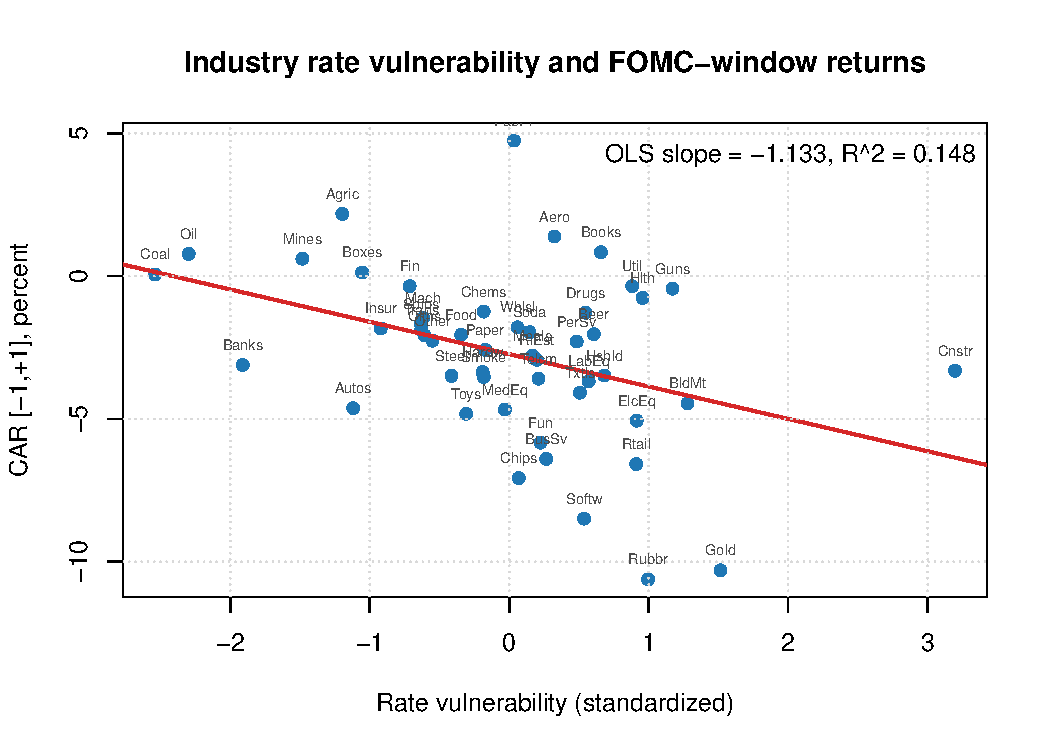
\includegraphics[width=0.78\textwidth]{../output/step1/step1_scatter_ols.pdf}
\caption{简单截面 OLS：利率脆弱度与事件窗口收益}
\label{fig:step1_scatter_ols}
\end{figure}

图 \ref{fig:step1_scatter_ols} 展示了简单利率脆弱度与事件窗口收益之间的负向关系。该图说明，一元截面中确实存在较明显的线性相关，但散点分布也显示行业间收益差异并非完全由单一变量解释，因此仍需要进一步控制行业风险暴露和收益特征。

不过，这个一元结果只能作为初步证据。原因在于上述 $RateVulnerability_i$ 只来自行业收益对 $\Delta DGS2$ 的简单时间序列回归，没有同时控制市场因子和风格因子。为减少利率脆弱度本身可能混入的风格暴露，本文进一步构造条件利率脆弱度：在事件前估计窗口内，同时控制 Fama--French 五因子和 2 年期美债收益率变化：
\[
r_{it}-RF_t=\alpha_i+\beta_{M,i}MktRF_t+\beta_{S,i}SMB_t+\beta_{H,i}HML_t
+\beta_{R,i}RMW_t+\beta_{C,i}CMA_t+\beta_{r,i}\Delta DGS2_t+\eta_{it},
\]
并定义
\[
RateVulnerability_i=-\widehat{\beta}_{r,i}.
\]
使用这一条件口径后，无控制变量的一元模型中 $RateVulnerability_i^z$ 的系数只有 0.016，HC1 p 值为 0.978，$R^2$ 几乎为 0。这个对比说明，裸相关关系对利率脆弱度的构造方式敏感，不能把简单口径下的显著负相关直接当作最终结论。

这种差异恰好体现了讲义中关于误差项和遗漏变量的提醒：一元模型把所有其他行业特征都放入 $u_i$，如果这些因素同时影响 $CAR_i$ 且与利率脆弱度相关，一元系数就会混合多种机制。因而本文后续将 M2 多元模型作为本节主规格，而把简单 OLS 作为研究起点和对照基准。

\subsection{增加控制变量后的拓展模型}
\label{subsec:multivariate_ols}

为缓解可观测遗漏变量带来的偏误，本文在单事件截面中逐步加入行业风险暴露和历史收益特征。多元基准模型写为
\[
CAR_i=\beta_0+\beta_1 RateVulnerability_i^z+\boldsymbol{\gamma}'\mathbf{X}_i+u_i,
\]
其中 $\mathbf{X}_i$ 包括市场 beta、Fama--French 风格因子 beta、历史波动率和事件前动量。模型组如下。

\begin{itemize}
  \item M0：只加入条件利率脆弱度 $RateVulnerability_i^z$。
  \item M1：在 M0 基础上加入市场 beta、历史波动率和事件前动量。
  \item M2：在 M1 基础上进一步加入 SMB、HML、RMW、CMA 风格因子暴露，是本节主规格。
\end{itemize}

M1 控制最基本的行业风险特征。市场 beta 用于吸收行业随市场整体波动的敏感性；历史波动率用于控制行业自身风险水平；事件前动量用于控制公告前价格趋势和预期交易。M2 则进一步纳入 Fama--French 五因子中的规模、价值、盈利能力和投资风格暴露，使利率脆弱度系数不再简单反映成长/价值、盈利能力或投资风格差异。根据第三讲，多元回归系数的解释必须写成``其他变量保持不变''下的偏效应。因此，M2 中 $\beta_1$ 的含义是：在市场 beta、SMB/HML/RMW/CMA beta、历史波动率和事件前动量相同的行业之间，利率脆弱度提高 1 个标准差时，事件窗口 $CAR$ 的平均差异。

表 \ref{tab:direct_main_results} 汇总了关键结果。可以看到，M0 中条件利率脆弱度几乎没有解释力；M1 中系数转为负但不显著；加入完整 Fama--French 风格暴露后，M2 的核心系数为 $-1.098$，常规 p 值为 0.0133，HC1 p 值为 0.0094，$R^2$ 提高到 0.565。进一步使用异方差稳健推断思想，采用更保守的 HC3 标准误后，M2 的 p 值为 0.0472，仍在 5\% 水平附近显著。

\begin{table}[H]
\centering
\caption{直接影响分析的主要截面回归结果}
\label{tab:direct_main_results}
\begin{threeparttable}
\begin{tabularx}{\textwidth}{p{0.15\textwidth}Xrrrr}
\toprule
模型 & 变量口径与控制变量 & 系数 & HC1 p 值 & HC3 p 值 & $R^2$ \\
\midrule
简单 OLS & 简单利率脆弱度；无控制变量 & -1.133 & 0.0068 & -- & 0.148 \\
M0 & 条件利率脆弱度；无控制变量 & 0.016 & 0.9781 & -- & 0.000 \\
M1 & M0 + 市场 beta、历史波动率、事件前动量 & -0.268 & 0.4955 & -- & 0.361 \\
M2 & M1 + SMB/HML/RMW/CMA 风格 beta & -1.098 & 0.0094 & 0.0472 & 0.565 \\
\bottomrule
\end{tabularx}
\begin{tablenotes}
\small
\item 注：因变量为 2022 年 11 月 2 日 FOMC 事件窗口 $[-1,+1]$ 的行业累计收益，单位为百分比。简单 OLS 使用只控制 $\Delta DGS2$ 的利率脆弱度；M0--M2 使用在事件前窗口内同时控制 Fama--French 五因子和 $\Delta DGS2$ 得到的条件利率脆弱度。HC3 p 值仅对 M2 主模型报告，用作小样本稳健推断口径。
\end{tablenotes}
\end{threeparttable}
\end{table}

M2 的结果支持直接影响假设的条件版本，即前文的 H2 偏效应假设：在控制行业风险暴露和历史收益特征后，利率脆弱度仍与 FOMC 事件窗口收益显著负相关。系数 $-1.098$ 表示，条件利率脆弱度每提高 1 个标准差，三日行业累计收益平均降低约 1.10 个百分点。由于全部解释变量均使用事件日前的历史窗口估计，控制变量不会使用事后信息。需要强调的是，这一结果仍应表述为控制可观测行业特征后的偏相关或偏效应，而不是不加限制地宣称严格因果效应；不可观测的行业现金流久期、融资约束、安全资产属性或事件日特殊新闻仍可能进入误差项。

从控制变量本身看，M2 中 SMB beta 系数为 1.764，HC1 p 值为 0.0014；事件前动量系数为 1.427，HC1 p 值为 0.0279；历史波动率系数为 $-1.415$，HC1 p 值为 0.1238。这个组合说明，事件窗口收益差异不仅由利率脆弱度解释，也与行业风格暴露和公告前收益趋势有关。正因为这些变量在 M2 中有较强解释力，直接使用一元模型会过度依赖误差项的外生性假定。多元 OLS 在这里的作用就是把可测度的行业风险特征显式纳入模型，降低遗漏变量偏误的风险。

\subsection{偏效应解释与模型设定检查}
\label{subsec:partial_effect_checks}

第三讲在讲解多元回归时强调，控制变量不是为了机械提高 $R^2$，而是为了使核心变量的系数具有更清楚的偏效应含义。本节围绕 M2 主模型报告四类设定检查：FWL 偏效应检查、多重共线性诊断、变量重要性比较和嵌套模型检验。

第一，FWL 检查显示，完整 M2 模型中 $RateVulnerability_i^z$ 的系数为 $-1.097882$，残差化后回归得到的 FWL 系数同样为 $-1.097882$。这意味着 M2 的核心结果可以被直观理解为：在剔除市场 beta、风格 beta、历史波动和事件前动量所能解释的部分后，利率脆弱度的剩余差异仍然能够解释行业 $CAR$ 的剩余差异。这个结果和第三讲关于``扣除其他变量解释部分后的净关系''完全一致。

\begin{figure}[H]
\centering
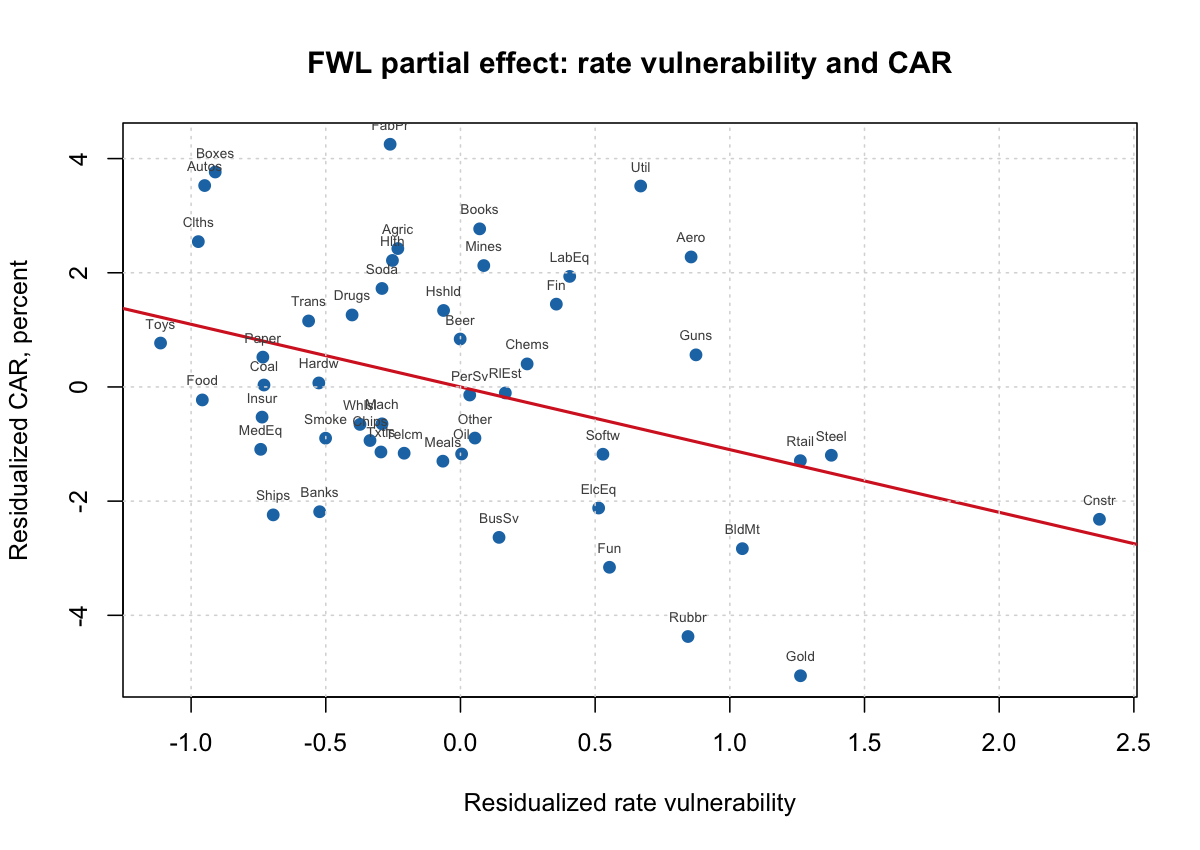
\includegraphics[width=0.78\textwidth]{../output/step3/fig_scatter_partial_effect.png}
\caption{FWL 偏效应图：残差化利率脆弱度与残差化 CAR}
\label{fig:fwl_partial_effect}
\end{figure}

图 \ref{fig:fwl_partial_effect} 进一步给出了偏效应的图示证据。横轴为剔除其他控制变量后剩余的利率脆弱度，纵轴为剔除同一组控制变量后剩余的事件窗口收益；拟合线仍然向下，说明 M2 的负向系数并不是简单由市场 beta、风格暴露、历史波动或事件前动量机械驱动。

第二，多重共线性诊断表明，M2 中 $RateVulnerability_i^z$ 的 VIF 为 1.90，最高 VIF 来自历史波动率，约为 6.60；RMW beta 的 VIF 约为 6.00。第三讲指出，可以用容忍度或 VIF 衡量解释变量之间的共线性，通常 VIF 大于 10 或容忍度小于 0.1 才认为多重共线性较强。本文所有变量的 VIF 均低于 10，说明共线性会增加部分估计量方差，但还不足以否定 M2 的可用性。尤其是核心变量 $RateVulnerability_i^z$ 的 VIF 较低，表明它并没有被其他控制变量严重线性解释。

第三，标准化系数用于比较不同解释变量的重要性。M2 中绝对值最大的标准化系数依次为 SMB beta (0.598)、事件前动量 (0.484)、历史波动率 ($-0.480$)、利率脆弱度 ($-0.372$) 和 RMW beta ($-0.357$)。这说明利率脆弱度不是唯一解释变量，但在完整控制变量体系中仍属于重要变量之一。其标准化系数为负，也与本文关于紧缩性利率冲击压低高脆弱行业收益的理论预期一致。

\begin{figure}[H]
\centering
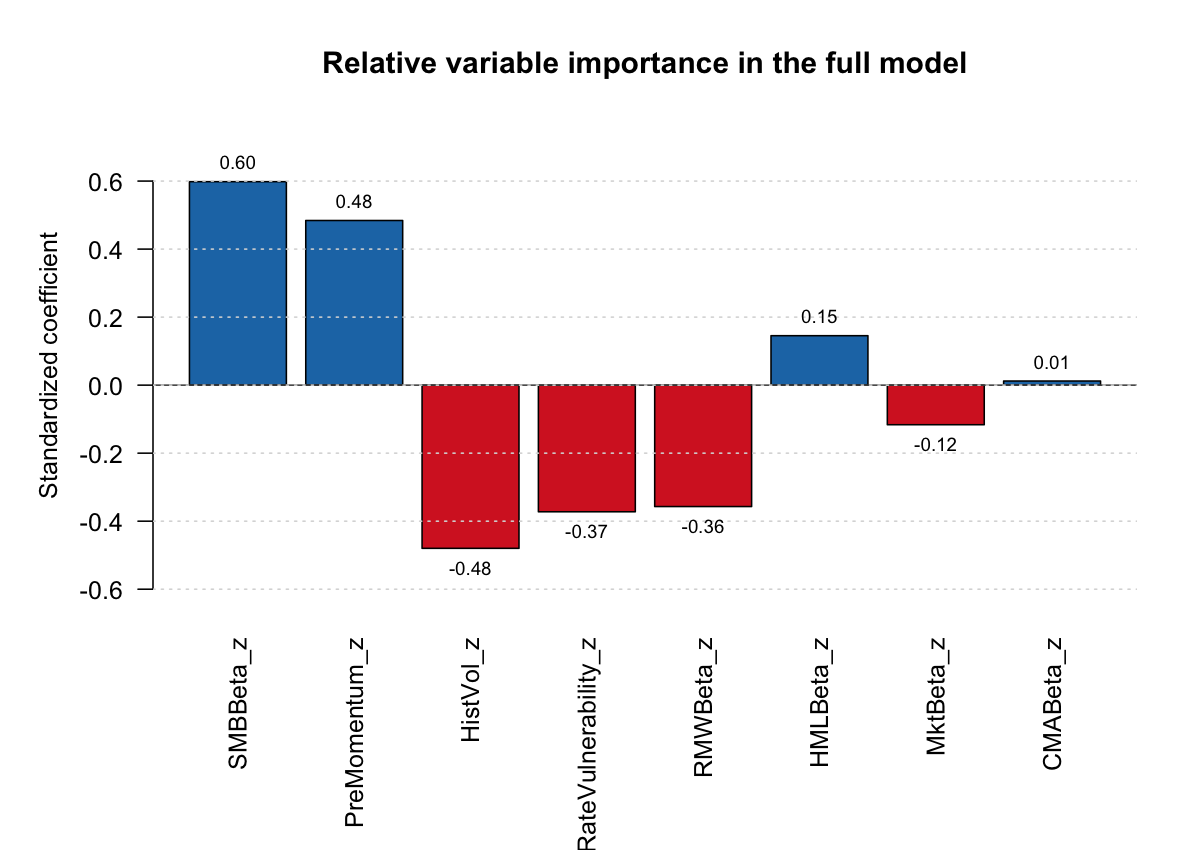
\includegraphics[width=0.78\textwidth]{../output/step3/fig_standardized_coefficients.png}
\caption{M2 主模型的标准化系数比较}
\label{fig:standardized_coefficients}
\end{figure}

图 \ref{fig:standardized_coefficients} 表明，M2 中事件前动量、SMB beta 和历史波动率等变量也具有较强解释力。这一点反过来说明，多元控制并非形式上的复杂化，而是必要的模型设定：若不控制这些变量，利率脆弱度系数可能混入行业风格和短期收益趋势的影响。

\begin{table}[H]
\centering
\caption{M2 主模型的设定检查}
\label{tab:m2_diagnostics}
\begin{threeparttable}
\begin{tabularx}{\textwidth}{p{0.27\textwidth}p{0.18\textwidth}X}
\toprule
检查项目 & 结果 & 含义 \\
\midrule
FWL 偏效应检查 & $-1.097882$ & 残差化系数与完整 M2 系数完全一致，支持偏效应解释。 \\
核心变量 VIF & 1.90 & $RateVulnerability_i^z$ 未被其他控制变量严重线性解释。 \\
最高 VIF & 6.60 & 最高值来自历史波动率，低于 10 的常用警戒线。 \\
M0 vs M2 联合 F 检验 & $F=7.436$, $p<0.001$ & 完整控制变量整体显著提高模型解释力。 \\
FF 风格 beta 联合 F 检验 & $F=4.708$, $p=0.0033$ & SMB/HML/RMW/CMA 风格暴露应进入主模型。 \\
利率脆弱度二次项 & $p=0.9840$ & 未发现需要加入简单二次项的证据。 \\
RESET 型检验 & $p=0.4041$ & 未发现明显函数形式误设证据。 \\
\bottomrule
\end{tabularx}
\begin{tablenotes}
\small
\item 注：FWL 检查、VIF 和嵌套 F 检验均基于 M2 主模型及相应辅助回归；RESET 型检验用于检查简单函数形式误设。
\end{tablenotes}
\end{threeparttable}
\end{table}

第四，嵌套模型 F 检验支持 M2 作为主规格。M0 与 M1 的比较显示，市场 beta、历史波动率和事件前动量联合显著，$F=8.282$，p 值为 0.00018；M0 与 M2 的比较显示，完整控制变量联合显著，$F=7.436$，p 值约为 $1.01\times 10^{-5}$；从 M1 到 M2 的比较显示，Fama--French 风格 beta 联合显著，$F=4.708$，p 值为 0.0033。因此，M2 不是为了追求更高的 $R^2$ 而任意加入变量，而是有资产定价理论基础并受到嵌套模型检验支持的主规格。

此外，本文还估计了行业组交互模型，用 TechGrowth、Finance 和 Defensive 三类行业组检验利率脆弱度斜率是否存在异质性。这里的 M3 full 模型不是新的主模型，而是在 M2 完整控制变量基础上，加入三类行业组虚拟变量及其与 $RateVulnerability_i^z$ 的交互项：
\[
\begin{aligned}
CAR_i
=&\ \beta_0+\beta_1 RateVulnerability_i^z+\boldsymbol{\gamma}'\mathbf{X}_i
+\theta_1 TechGrowth_i+\theta_2 Finance_i+\theta_3 Defensive_i\\
&+\lambda_1(RateVulnerability_i^z\times TechGrowth_i)
+\lambda_2(RateVulnerability_i^z\times Finance_i)
+\lambda_3(RateVulnerability_i^z\times Defensive_i)+u_i .
\end{aligned}
\]
因此，M3 full 中“三个斜率交互项联合 p 值为 0.0917”检验的是原假设
\[
H_0:\lambda_1=\lambda_2=\lambda_3=0,
\]
也就是科技成长、金融和防御性行业是否共同改变了利率脆弱度与事件窗口收益之间的斜率关系。它不是检验 M3 模型整体是否显著，也不是检验这三类行业的平均收益是否不同。

常规 F 检验下三个斜率交互项联合 p 值为 0.0917，说明在 10\% 水平附近存在一定行业组斜率异质性证据，但在 5\% 水平下并不强。使用 HC1 稳健 Wald 检验时，三个交互项联合 p 值为 0.0013，显示稳健协方差口径下行业组斜率差异更明显。单项结果显示，Finance 和 Defensive 交互项为正，意味着这些行业组中利率脆弱度的负向斜率可能被部分抵消，或者其反应机制不同于其他行业。由于样本只有 49 个行业，加入行业组虚拟变量和交互项会明显消耗自由度，且不同检验口径下显著性不完全一致，因此本文将 M3 结果作为后文异质性分析的补充线索，不取代 M2 作为直接影响分析的主结论。

\subsection{本节小结}
\label{subsec:direct_summary}

综合来看，本节得到三点结论。第一，简单 OLS 显示，标准化利率脆弱度与 2022 年 11 月 2 日 FOMC 事件窗口收益显著负相关，系数约为 $-1.133$。第二，这一一元关系对变量构造敏感：改用同时控制 Fama--French 五因子的条件利率脆弱度后，M0 系数约为 0.016 且完全不显著。因此，简单回归只能作为起点，不能作为最终结论。第三，加入完整行业风险暴露和历史收益控制后，M2 中 $RateVulnerability_i^z$ 的系数约为 $-1.098$，HC1 p 值为 0.0094，HC3 p 值为 0.0472，说明在控制可观测行业特征后，高利率脆弱行业在紧缩性 FOMC 事件中表现更弱。

因此，本节的核心结论是：在该次紧缩性 FOMC 公告窗口中，高利率脆弱行业的表现显著更弱，而且这一关系在控制主要可观测行业风险特征后仍然存在。根据讲义中的零条件均值思想，多元 OLS 已经控制了可测度的遗漏变量，但如果仍存在不可观测且与利率脆弱度相关的行业特征，$\beta_1$ 仍可能受到内生性影响。这个问题将在后文内生性与 IV/2SLS 部分继续讨论。


% =======================
% 5 模型诊断与稳健性检验
% =======================
\section{模型诊断与稳健性检验：异方差、影响点与替代估计}

\subsection{异方差的实际原因与统计检验}

% 实际原因：不同行业波动率、融资结构、避险属性不同。
% 统计检验：
% Breusch-Pagan p 约 0.346，
% modified White p 约 0.196，
% full White p 约 0.310。
% 口径：统计上未拒绝同方差，但小样本和行业差异使 HC3 更稳妥。

\subsection{稳健标准误、WLS与FGLS}

% 写 HC3、WLS、FGLS、FGLS-White。
% 主口径：WLS/FGLS 是稳健性，不替代 OLS-HC3。

\subsection{影响点与leave-one-out}

% Gold 是最大影响点。
% 全样本 HC3：-1.098，p 约 0.047。
% 剔除 Gold：-0.738，p 约 0.113。
% 剔除 Cook 距离前三行业：-0.563，p 约 0.229。
% 口径：方向稳健，显著性受高影响行业影响。

% =======================
% 6 内生性分析
% =======================
\section{内生性分析：遗漏变量、测量误差与IV/2SLS}

\subsection{内生性来源}

% 遗漏变量：行业久期、融资约束、安全资产属性、宏观风险暴露。
% 测量误差：利率脆弱度是 generated regressor。
% 反向因果：较弱，但共同冲击仍需讨论。

\subsection{代理变量检验}

% 写 GoldDummy、HighGrowthProxy、HighVolProxy、FinanceDummy、DefensiveDummy。
% 说明代理变量加入后核心方向多数仍为负，但 GoldDummy 使显著性下降。

\subsection{工具变量与2SLS}

% 写 Z_precovid_2Y_z 第一阶段 F 约 16.42，partial R2 约 0.291。
% 2SLS 系数约 -1.812，p 约 0.302。
% DWH p 约 0.286。
% 过度识别 p 值约 0.109--0.237。
% 口径：IV 方向一致但不显著，是辅助证据，不替代 OLS-HC3。

% =======================
% 7 异质性与影响机制分析
% =======================
\section{异质性与影响机制分析：面板、DID/DDD与风险状态}

\subsection{行业异质性：行业组交互项}

% 写 Finance、Defensive、TechGrowth 交互项。
% 口径：行业属性会改变利率脆弱度与FOMC收益反应之间的关系，但交互结果作为补充。

\subsection{政策环境异质性：多事件TWFE与2022快速加息}

% 连续暴露 TWFE 系数约 -0.149，p 约 0.063。
% shock_x_vulnerability:tightening_2022 系数约 -0.0755，p 接近 0。
% 解释为：2022快速加息阶段，高利率脆弱行业受到更强负向冲击。

\subsection{公告窗口机制：DID/DDD}

% 即时 [0,+1] x hawkish DDD 系数约 -0.135，p 约 0.108。
% 完整 [0,+5] 后窗 DDD 更弱。
% 说明市场利率冲击定义的 hawkish surprise 比实际 hike 更贴近资产定价反应。

\subsection{下行风险机制：限值因变量模型}

% LPM：rv_hawkish 约 0.0475，p 约 0.0226。
% Logit/Probit 平均偏效应约 0.0484/0.0471。
% Poisson：rv_hawkish 约 0.0241，p 约 0.0443。
% Tobit：rv_hawkish 约 0.276，p 约 0.00047。
% 解释为：高利率脆弱行业在鹰派公告后不仅平均收益更弱，也更容易进入下行风险状态。

% =======================
% 8 方法扩展：住房市场SEM
% =======================
\section{方法扩展：联立方程视角下的住房市场供需系统}

\subsection{为什么不把FOMC行业CAR强行写成SEM}

% 行业 CAR 与历史利率脆弱度不是标准同时均衡系统。
% 本节只是方法扩展，不作为行业收益主证据。

\subsection{住房市场供需结构方程}

% 需求方程：销售量由价格、抵押贷款利率、收入、失业率解释。
% 供给方程：销售量由价格、建筑许可、月供给量、建筑成本解释。

\subsection{2SLS与识别诊断}

% 需求方程第一阶段 F 约 78.64。
% 供给方程第一阶段 F 约 70.03。
% 但过度识别检验拒绝、核心价格系数不稳定、非平稳问题存在。
% 口径：展示联立方程识别条件的重要性，不作为强因果证据。

% =======================
% 9 政策含义与实践启示
% =======================
\section{政策含义与实践启示}

\subsection{对货币政策沟通的启示}

% FOMC政策冲击不是只影响市场平均收益，而会在行业间产生差异化反应。
% 政策沟通应减少不必要的预期误差，并关注金融市场的行业结构性反应。
% 注意：不要写成“美联储应该为了某些行业改变利率政策”。

\subsection{对金融监管和风险监测的启示}

% 监管部门和风险监测者不应只看大盘指数反应。
% 应跟踪行业层面的利率暴露和下行风险指标。
% 限值因变量模型显示，鹰派公告后高脆弱行业更容易跑输并出现下行损失。

\subsection{对投资者和资产配置的启示}

% 投资者在FOMC会议前后不应只判断“加息或降息”。
% 还要区分实际政策动作和市场利率 surprise。
% 行业组合配置应关注利率脆弱度、历史波动和事件前动量。

\subsection{对实体经济传导的启示}

% 住房 SEM 表明，在实体部门中利率传导可能表现为价格和数量的共同调整。
% 该部分仅作为传导机制启示，不作为精确政策评估。

% =======================
% 10 Conclusion
% =======================
\section{Conclusion：结论与不足}

% 第一段：回答研究问题。
% 第二段：概括主要发现。
% 第三段：政策含义总结。
% 第四段：不足与未来研究。
%
% 不足：
% 1. 样本行业数有限。
% 2. Gold 等高影响行业影响显著性。
% 3. IV 排除限制依赖经济论证，2SLS 不显著。
% 4. FOMC 短窗口仍可能混入其他新闻。
%
% 未来研究：
% 使用高频货币政策 surprise、公司层面数据、行业杠杆、现金流久期和融资约束指标进一步检验机制。

% =======================
% 参考文献
% =======================
\section{cite}


\begin{thebibliography}{99}

\bibitem[Kuttner(2001)]{kuttner2001monetary}
Kuttner, K. N. (2001).
Monetary policy surprises and interest rates: Evidence from the Fed funds futures market.
\textit{Journal of Monetary Economics}, 47(3), 523--544.

\bibitem[Bernanke and Kuttner(2005)]{bernanke2005stock}
Bernanke, B. S., and Kuttner, K. N. (2005).
What explains the stock market's reaction to Federal Reserve policy?
\textit{The Journal of Finance}, 60(3), 1221--1257.

\bibitem[G{\"u}rkaynak et al.(2005)]{gurkaynak2005actions}
G{\"u}rkaynak, R. S., Sack, B., and Swanson, E. T. (2005).
Do actions speak louder than words? The response of asset prices to monetary policy actions and statements.
\textit{International Journal of Central Banking}, 1(1), 55--93.

\bibitem[Fama and French(1993)]{fama1993common}
Fama, E. F., and French, K. R. (1993).
Common risk factors in the returns on stocks and bonds.
\textit{Journal of Financial Economics}, 33(1), 3--56.

\bibitem[Fama and French(2015)]{fama2015five}
Fama, E. F., and French, K. R. (2015).
A five-factor asset pricing model.
\textit{Journal of Financial Economics}, 116(1), 1--22.

\bibitem[Cochrane(2005)]{cochrane2005asset}
Cochrane, J. H. (2005).
\newblock \textit{Asset Pricing}.
\newblock Revised edition. Princeton University Press, Princeton and Oxford.

\bibitem[Mishkin(1996)]{mishkin1996channels}
Mishkin, F. S. (1996).
\newblock The channels of monetary transmission: Lessons for monetary policy.
\newblock NBER Working Paper No. 5464. National Bureau of Economic Research.

\bibitem[Bernanke and Gertler(1995)]{bernanke1995inside}
Bernanke, B. S., and Gertler, M. (1995).
\newblock Inside the black box: The credit channel of monetary policy transmission.
\newblock \textit{Journal of Economic Perspectives}, 9(4), 27--48.

\bibitem{kenFrench49Daily}
Kenneth R. French Data Library.
\newblock 49 Industry Portfolios Daily.
\newblock \url{https://mba.tuck.dartmouth.edu/pages/faculty/ken.french/ftp/49_Industry_Portfolios_daily_CSV.zip}.

\bibitem{kenFrenchFF5Daily}
Kenneth R. French Data Library.
\newblock Fama--French Research Data 5 Factors (2x3) Daily.
\newblock \url{https://mba.tuck.dartmouth.edu/pages/faculty/ken.french/ftp/F-F_Research_Data_5_Factors_2x3_daily_CSV.zip}.

\bibitem{federalReserveH15}
Board of Governors of the Federal Reserve System.
\newblock H.15 Selected Interest Rates.
\newblock \url{https://www.federalreserve.gov/datadownload/Choose.aspx?rel=H15}.

\bibitem{fredDGS2}
Federal Reserve Bank of St. Louis.
\newblock Market Yield on U.S. Treasury Securities at 2-Year Constant Maturity, Quoted on an Investment Basis (DGS2).
\newblock \url{https://fred.stlouisfed.org/graph/fredgraph.csv?id=DGS2}.

\bibitem{federalReserveFOMCCalendar}
Board of Governors of the Federal Reserve System.
\newblock FOMC calendars and statements.
\newblock \url{https://www.federalreserve.gov/monetarypolicy/fomccalendars.htm}.

\bibitem{federalReserveFOMC20221102}
Board of Governors of the Federal Reserve System.
\newblock Federal Reserve issues FOMC statement, November 2, 2022.
\newblock \url{https://www.federalreserve.gov/newsevents/pressreleases/monetary20221102a.htm}.

\bibitem{fredHousingSeries}
Federal Reserve Bank of St. Louis.
\newblock FRED housing-market monthly series used in the simultaneous-equations extension: HSN1F, MSPNHSUS, MORTGAGE30US, DSPIC96, UNRATE, PERMIT, MSACSR, WPUSI012011, HOUST, and UNDCONTSA.
\newblock \url{https://fred.stlouisfed.org/}.

\end{thebibliography}

\end{document}
